\chapter{Introduction} \label{ch:intro}
A guiding principle in the study of physics is that of limiting behavior.
When approaching any new problem or system, a great deal of insight may be achieved by first considering the most extreme examples.
In the case of atomic physics, the pursuit of extremely low-energy gases has proven to be an incredibly fruitful endeavor, resulting in some of the most rigorously tested and well understood theories to date \hl{lamb shift}.
Furthermore, ultracold and quantum degenerate neutral gases allow us to consider the quantum nature of matter, and its interaction with externals fields, in the few-body and many-body regimes \hl{ref on neutral gases?}.

Rapid advancement in the ability to laser cool and trap atoms \hl{ref} has led to a number of notable achievements including the creation of novel macroscopic states of quantum matter such as Bose-Einstein condensates (BEC) and degenerate Fermi gases \cite{aem95,Bradley1995,dma95,DeMarco1999,zhg03,MartinezdeEscolar2010,Mickelson2010ja,dym10a,stg10}, the observation of the BEC-BCS crossover and quantum phase transitions \cite{rgj04,zss04,cba04Science,Bourdel2004,grj03,Greiner2002,jsg08,Snoke2002,zbb14}, as well as the formation of macroscopic ensembles of ro-vibrational ground state molecules \cite{rtb03,Jones2006, Reinaudi2012,Stellmer2012,nom08,Lang2008}.

Each of these successes has been enabled by the precise control and tunability of interactions between atoms using external fields.
A common use of coupling the internal states of atoms using optical fields is the process of photoassociation, whereby colliding atoms, illuminated by resonant laser light, absorb photons and associate to form a bound molecule \cite{Kohler2006, Jones2006, Chin2010}.
This process is illustrated in Fig.\,\ref{fig:1pasSch}.
\begin{figure} 
	\centerline{
	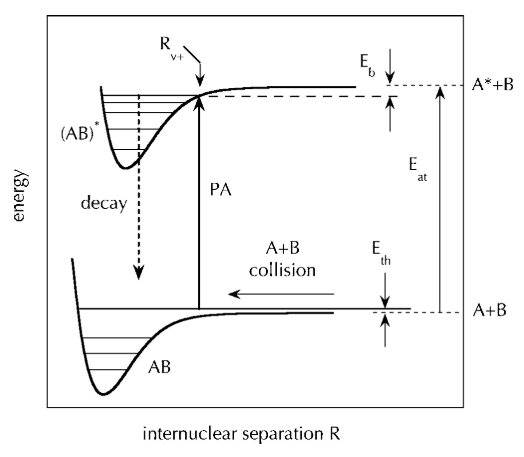
\includegraphics[width=0.7\textwidth]{model_PAS.PNG}}
	\caption{Schematic of the photoassociation process}{}
	\label{fig:1pasSch}
\end{figure}
The process shown in this figure involves a single-photon and is known as one-photon photoassociation.
Absorption of the single-photon will promote one atom of the colliding pair to an excited state that results in the creation of an excited weakly-bound molecular state when the laser frequency is appropriately tuned.
The formation of this molecule is subsequently followed by spontaneous or stimulated decay, typically resulting in loss of both atoms from the trap.
Detection of this atom loss is commonly observed as evidence of photoassociation.

Photoassociation of free atoms results in the creation of weakly-bound molecular states due to the long-range nature of the scattering wavefunctions which preferentially overlap with molecular states having large spatial extent \hl{ref}.


By starting with the photoassociation laser frequency slightly detuned from the free-atom asymptote and scanning to the red, a series of resonances progressively further from the free atom excited state may be observed.
These resonances correspond to excitation of progressively more deeply bound molecules within the excited state potential well.
For small binding energies, the molecules largely share the characteristics of the constituent free atoms, while more deeply bound molecules begin exhibiting splittings and couplings unique to the interactions and symmetries which make up the potential \hl{PA review ref}.

Since we can directly measure the binding energy of molecules with PAS, this process reveals details about the interaction potential and may be used as a tool for finding parameters such as the scattering length of free atom atomic species \hl{refs}.
Alternatively, by adding an additional light field, two-photon photoassociation may be used to populate excited molecular states of the ground state potential.
This technique has proven to be an incredibly precise way to discern information about the collisional properties of ultracold atomic gases \hl{ref on two photon} \cite{MartinezDeEscobar2008}.

However, the direct coupling of free atoms to the most deeply bound molecular states is not a favorable process and generally requires the use of additional photoassociative steps.
These may include STIRAP or preferential decay from excited-molecular states as has been recently demonstrated \cite{Reinaudi2012, cbc17, Stellmer2012, Ciamei2017}.
Ro-vibrational ground state molecules are interesting as their use has been proposed for precision measurements of deviations of the proton-electron mass ratio \cite{zky08, Kotochigova2009} and the fine structure constant \cite{Beloy2011}. 

For some atomic species, external magnetic fields may also be used to create weakly bound molecular states through the use of magnetic Feshbach resonances \cite{Kohler2006, Chin2010}.
These scattering resonances are the result of coupling between energetically accessible scattering states (called open channels) and energetically inaccessible bound states (closed channels) where the scattering and bound states lie on two separate atomic interaction potentials with a differential magnetic moments.
When the closed channel is swept through the threshold energy of the open channel, a weakly bound molecular state known as a Feshbach molecule is formed \cite{cbk03, grj03,hkm03,rtb03,sph03}.
In the vicinity of the resonance position when the closed channel is just below threshold, these Feshbach molecules may explore a regime of universality where the wavefunction of the dressed molecular state extends far into the classically forbidden region.
These exotic long-range molecules are called halo molecules \cite{Kohler2006}.
These states may be characterized by large positive values of the free atom scattering length $a$ such that the binding energy of the halo molecule is given by
\begin{equation}
	E_b = -\frac{\hbar^2}{2 \mu a^2}
\end{equation}
where $\mu$ is the reduced mass of the atom pair.

\section{Halo molecules} \label{sec:halo}
The concept of a spatially extended, few-particle, halo system has found application in a number of fields including nuclear and molecular physics.
With the most well known examples being the deuteron and $^4$He$_2$ molecules \cite{lmk93,sto94,Kohler2006}.
In atomic physics, halo molecules exist as the least-bound state in the extreme case of a scattering resonance.
Such halo states exhibit spatially extended wavefunctions which reach well past the classical turning point, $r_\text{classical}=\left( \frac{2 \mu a^2 C_6}{\hbar^2} \right)^{1/6}$.
Fig.\,\ref{fig:86halo} shows the radial component of the $^{86}$Sr$_2$ halo wavefunction with farthest extent $>\!1000$\,a$_0$, where a$_0$ is the Bohr radius.
\begin{figure}
	\centerline{
	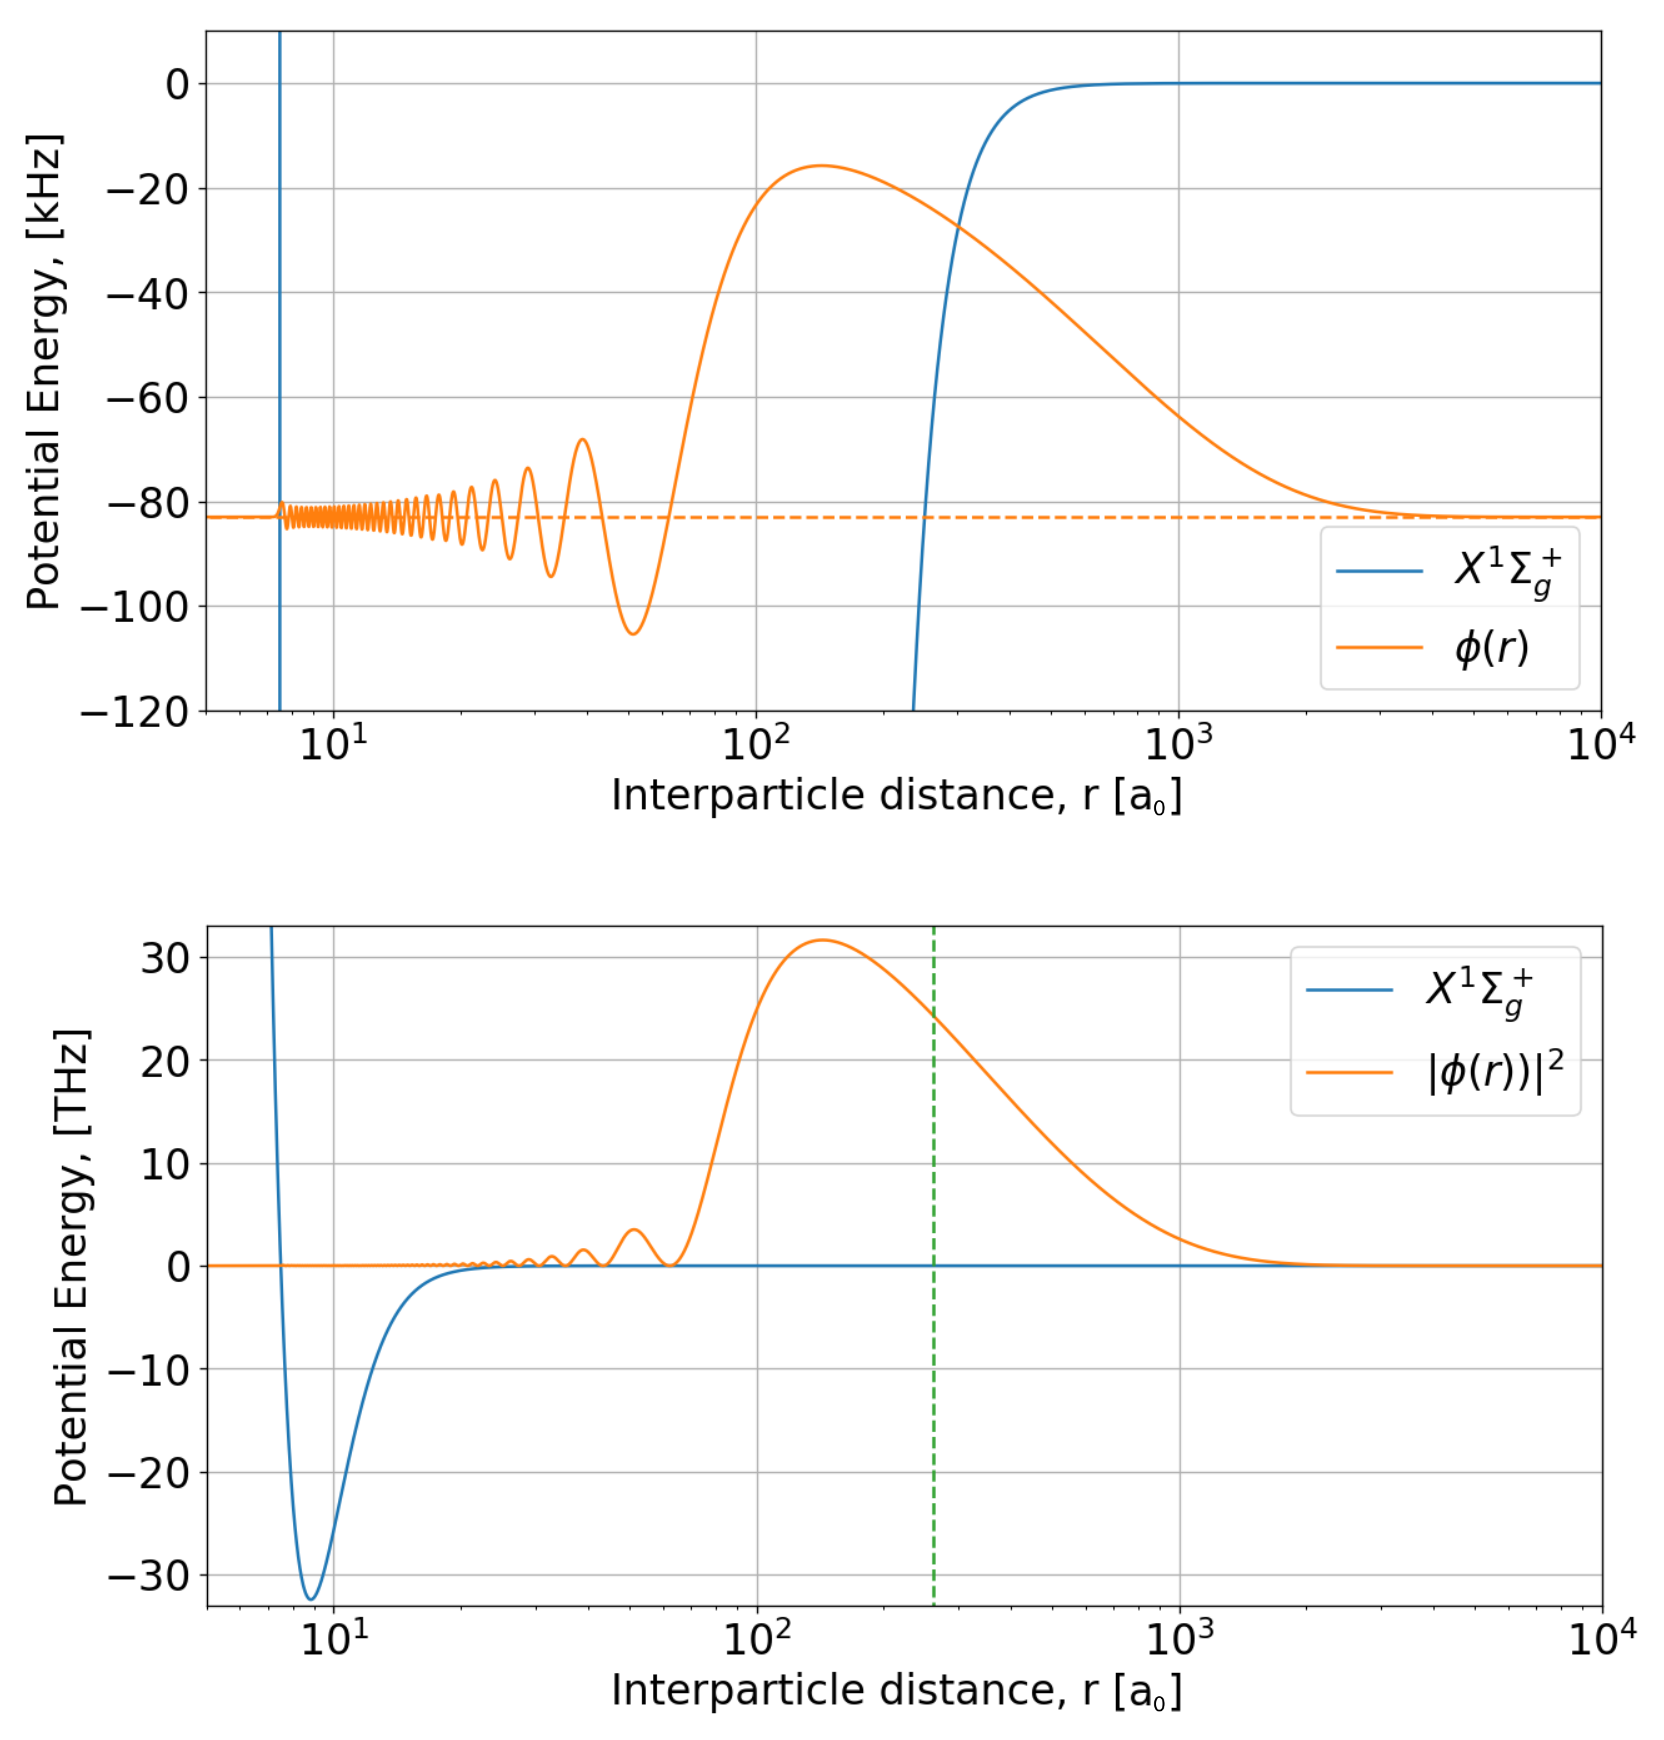
\includegraphics[width=\textwidth]{86halo.png}}
	\caption{$^{86}$Sr$_2$ halo radial wavefunction}{The strontium-86 halo wavefunction is calculated using the Johnson renormalized Numerov method \cite{Gibson2016, Johnson1978} and the X$^1\Sigma_g^+$ potential from Ref.\,\cite{Stein2010}. The vertical dashed line is placed at the classical turning point $r_\text{classical} \approx 260$\,a$_0$. Note, the wavefunction normalization here is arbitrary and only for illustrative purposes.}
	\label{fig:86halo}
\end{figure} 
Halo molecules are characterized by their universality, meaning that molecular properties such as size and binding energy can be parameterized by a single quantity, the $s$-wave scattering length $a$, independent of other details of the atom-pair interaction \cite{Kohler2006,bha06}. 
Additionally, Efimov trimers may also exist in systems near a scattering resonance, influencing dimer and atomic scattering properties and introducing additional universal phenomena \cite{bha07,nen17}.

Ultracold halo molecules are often associated with magnetic Feshbach resonances \cite{Chin2010}.
However, in this work, we probe a naturally occurring halo state which exists in the absence of tuning with a magnetic Feshbach resonance. 
This extremely weakly-bound molecular state depends strongly on the long-range portion of the interaction potential between atoms and therefore, measurement of the binding energy should provide a precise estimate of the long-range $C_6$ coefficient.

There are important differences between halo molecules associated with magnetic Feshbach resonances and the naturally occurring halo molecule in $^{86}$Sr. 
With magnetic Feshbach resonances, the relevant scattering and bound molecular states lie on different molecular potentials, and single-photon magnetic-dipole transitions can be used to measure molecular binding energies with RF or microwave spectroscopy \cite{Chin2010,cju05,thw95b}. 
Typically, this is done by first forming molecules through magneto-association and then driving bound-free or bound-bound transitions converting the halo molecule into a different state. 
Other methods include spectroscopy with an oscillating magnetic field \cite{thw95b}, a modulated optically controlled Feshbach resonance \cite{chx15}, and Ramsey-type measurements of atom-molecule oscillation frequencies \cite{ckt03}. 
It is also possible to efficiently populate halo states with evaporative cooling \cite{jba03} near a magnetic Feshbach resonance. 
These are powerful techniques for manipulating quantum gases of alkali metals and other open-shell atoms, for which there are many magnetic Feshbach resonances. 
Strontium, however, due to its closed-shell electronic structure, lacks magnetic Feshbach resonances in the electronic ground state.

\section{Properties of strontium}
\label{sec:sr}
Strontium is an alkaline-earth element with four naturally occurring isotopes, three bosonic and one fermionic.
The two valence electrons in its outer shell may align their spin anti-parallel or parallel, giving rise to a singlet and triplet series, respectively, of optical transitions.
Thus, two laser cooling phases are required to cool strontium to $\approx\!1\,\mu$K.
The first using the strong dipole-allowed $^1S_0\,\rightarrow\,^1P_1$ transition at $461$\,nm and the second using the narrow intercombination line $^1S_0\,\rightarrow\,^3P_1$ transition at $689$\,nm \hl{older Sr refs}.
These laser cooling transitions, as well as required repumping transitions, are shown in Fig.\,\ref{fig:energyLevels}.
	\begin{figure} 
		\centerline{
		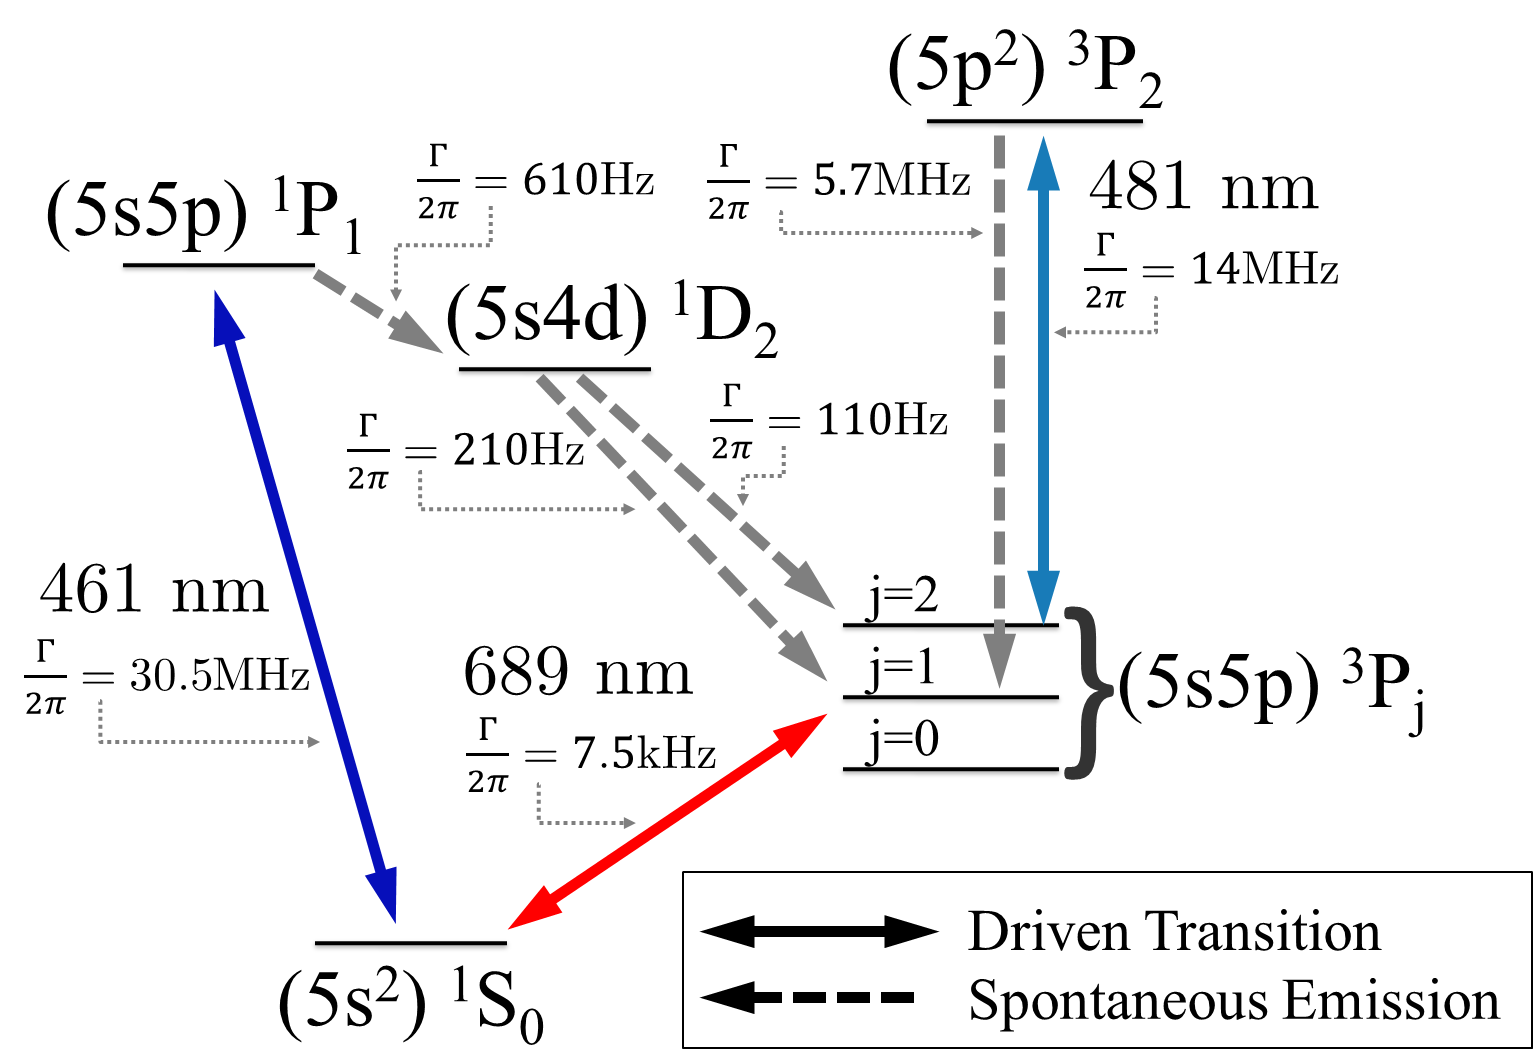
\includegraphics[height=0.45\textheight]{energy_level_diagram.png}}
		\caption{Partial energy level diagram of strontium}{Shown are the relevant transitions and decay rates utilized to perform laser cooling and spectroscopy.}
		\label{fig:energyLevels}
	\end{figure}
	
The isotopic differences in strontium have important implications for their use in certain experiments.
In particular, the bosonic isotopes of strontium $^{88}$Sr, $^{86}$Sr, and $^{84}$Sr have no nuclear spin, $\vec{I}=0$.
This lack of hyperfine structure results in a single ground state potential, which greatly simplifies the treatment of collisions and scattering for these atoms.
Conversely, the fermionic isotope $^{87}$Sr has a large nuclear spin $\vec{I}=9/2$, which when combined with the lack of electronic angular momentum in the ground state, results in a high degree of symmetry that must be considered when determining the behavior of these atoms during collisions.
This $SU(N)$ symmetry of $^{87}$Sr has led it to become a popular candidate for proposals exploring exotic phases of quantum magnetism \cite{Beverland2016,cre14,Chen2015}.

In addition to the differences in quantum statistics and shifts of transition frequencies between isotopes, the homonuclear $s$-wave scattering lengths range from $-2$a$_0$ for $^{88}$Sr to $\sim 800$a$_0$ for $^{86}$Sr.
From our measurement of the halo binding energy we derive estimates of these scattering lengths as given in Fig.\,\ref{fig:massScaling} \cite{Aman2018}.
Most importantly for this work, we use the isotope with the largest homonuclear scattering length, strontium-86.
These experiments utilize two-photon photoassociation performed near the narrow intercombination line $^1S_0\,\rightarrow\,^3P_1$ transition.
Similar work measuring the least-bound state of the X$^1\Sigma_g^+$ potential has been performed in $^{88}$Sr \cite{MartinezDeEscobar2008}.
Additionally, two-photon techniques have been used in optical lattices with $^{88}$Sr \cite{Reinaudi2012, McGuyer2014, McGuyer2015a, rom12} and $^{84}$Sr \cite{Stellmer2012} to produce excited bound state molecules in the electronic ground state.
One-photon photoassociation spectroscopy probing the excited state molecular binding energies has also been performed bulk trapped gases near the intercombination transition in $^{86}$Sr \cite{Borkowski2014a, Reschovsky} and $^{84}$Sr \cite{Stellmer2012, Reschovsky}.
The most abundant isotope, $^{88}$Sr, has been studied extensively in the context of narrow-line photoassociation, including one-photon PAS in a lattice \cite{Zelevinsky2006,McGuyer2013}, excitation of coherent Rabi oscillations between atomic and molecular condensates \cite{Yan2013b}, and the observation of optical Feshbach resonances \cite{Yan2013c, Blatt}.

\section{Thesis Outline} \label{sec:outline}
This thesis will describe our work probing the weakly bound halo state of strontium-86.
Chapter 2 will outline our standard laser cooling and trapping procedures for producing samples of ultracold strontium at $\approx1\,\mu$K in an optical dipole trap. 
Additionally, the experimental apparatus and systems for trapping will be discussed.
Chapter 3 will develop the theoretical underpinnings of the photoassociation process which has a rate dependent on the atomic spatial and thermal distribution in addition to the dynamical coupling provided by the applied PAS light fields.
Furthermore, this chapter explores atomic collisions and the importance of short-range interactions in determining the long-range behavior of scattering states.
In chapters 4 and 5, we present our findings from experiments probing the $^{86}$Sr$_2$ halo molecule.
The first experiments are performed in a strongly coupled regime where we observed non-linear loss features and AC Stark shifts on the order of the binding energy of the halo molecule.
Following this, we performed a complimentary set of experiments, being careful to stay in a weakly perturbing regime, where we precisely determined the binding energy of the halo molecule accounting for several different possible shifts of the resonance energy.
This binding energy is then used to estimate improved scattering lengths for all isotopes of strontium.
Chapter 6 describes the installation and characterization of a $532$\,nm lattice laser system.
This system will be indispensable for our future work investigating quantum magnetism with fermionic strontium-87 as well as studies aimed to control atomic interactions building from the photoassociative techniques developed in this thesis.
Further discussion of our proposed work will be given in chapter 7, along with concluding remarks.









%%%%%%%%%%%%%%%%%%%%%%%%%%%%%%%%%%%%%%%%%%%%%%%%%%%%%%%%%%%%%%%%%%%%%%%%%%%%%%%%%%%%%%%%%%%%%%%%%%%%%%%%%
%	
%This spatial discrimination along with the precise energy required to couple to a bound state result in a flexible tool mapping out the wavefunction of the scattering state to find its $s$-wave scattering length.
%
%
%Deeply bound molecular states are, in general, quite complicated and demonstrate a multitude of resonance frequencies between various internal, vibrational, and rotational energies.
%Photoassociation of free atoms 
%
%
%PA favors physicist molecules
%A significant part of the interest in ultracold AP has been the nature of the molecular states which are reafily produced and studied using this technique.
%The degree to which the atom molecule connection can be explicilty made in practice depdns aon the 
%high vibrational level are call long range molecules and prove one exmaple of a physicist molecules moleucles that can be related to the properties of the constituent atoms.
%
%In the most extreme case, molecules with binding energies of $10$
%
%
%modies atomic collisions
%
%yields information on atomic collisions
%field of photoassociation in ultracold gases, wherein studies of molecular structure have revealed the most accurate descriptions of atomic interactions and have become a fundamental probe of the ultracold toolbox \cite{Jones2006}.

%From this discussion, we 
%PA can come in many forms (in a lattice, in a bulk gas, via dissociating molecules) Experimentally we observe PA by looking for trap loss \hl{doublon paper}.
% 
% 
%rabi oscilations between atomic and molecular condensates (cite ours and the lattice experiment that followed)

%are the primary trapping mechanism for many alkali atom experiments and when combined with appropriately polarized and near resonant light a magneto-optical trap (MOT) is a robust tool applicable to nearly all cold atomic physics experiments.
%Furthermore, the use of dynamic B-fields allows researchers to tune atomic interactions at a microscopic level using

%Surprisingly, this phenomena may be described by simple two-level models and has become a mainstay in many atomic physics laboratories.
%
%While magnetic tuning may lend itself to simple theoretical descriptions, the temporal and spatial control of optical fields is unmatched.